\documentclass[15pt,a5paper,reqno]{article}
\usepackage{hyperref}
\usepackage[warn]{mathtext}
\usepackage[utf8]{inputenc}
\usepackage[T2A]{fontenc}
\usepackage[russian]{babel}
\usepackage{amssymb, amsmath, multicol}
\usepackage{graphicx}
\usepackage[shortcuts,cyremdash]{extdash}
\usepackage{wrapfig}
\usepackage{gensymb}
\usepackage{floatflt}
\usepackage{lipsum}
\usepackage{verbatim}
\usepackage{concmath}
\usepackage{euler}
\usepackage{xcolor}
\usepackage{etoolbox}
\usepackage{fancyhdr}
\usepackage{subfiles}
\usepackage{enumitem}
\usepackage{amsthm}
\usepackage{indentfirst}
\usepackage{import}

\DeclareMathOperator{\sign}{sign}

\RequirePackage[ left     = 1.5cm,
  right    = 1.5cm,
  top      = 2.0cm,
  bottom   = 1.25cm,
  includefoot,
  footskip = 1.25cm ]{geometry}
\setlength    {\parskip}        { .5em plus .15em minus .08em }
%\setlength    {\parindent}      { .0em }
\renewcommand {\baselinestretch}{ 1.07 }

\fancyhf{}

\renewcommand{\footrulewidth}{ .0em }
\fancyfoot[C]{\texttt{\textemdash~\thepage~\textemdash}}

\makeatletter
\patchcmd\l@section{%
  \nobreak\hfil\nobreak
}{%
  \nobreak
  \leaders\hbox{%
    $\m@th \mkern \@dotsep mu\hbox{.}\mkern \@dotsep mu$%
  }%
  \hfill
  \nobreak
}{}{\errmessage{\noexpand\l@section could not be patched}}
\makeatother
\parindent = 1cm % отступ при красной строке⏎
\pagestyle{fancy}    
\renewcommand\qedsymbol{$\blacksquare$}

\newcommand{\when}[2]{
  \left. #1 \right|_{#2} \hspace
}
\renewcommand{\kappa}{\varkappa}
\RequirePackage{caption2}
\renewcommand\captionlabeldelim{}
\newcommand*{\hm}[1]{#1\nobreak\discretionary{}

\DeclareSymbolFont{T2Aletters}{T2A}{cmr}{m}{it}
{\hbox{$\mathsurround=0pt #1$}}{}}
% Цвета для гиперссылок
\definecolor{linkcolor}{HTML}{000000} % цвет ссылок
\definecolor{urlcolor}{HTML}{799B03} % цвет гиперссылок
 
\hypersetup{pdfstartview=FitH,  linkcolor=linkcolor,urlcolor=urlcolor, colorlinks=true}


%\setcounter{secnum[utf8x]depth}{0}

\begin{document}

% НАЧАЛО ТИТУЛЬНОГО ЛИСТА
\begin{center}
  {\small ФЕДЕРАЛЬНОЕ ГОСУДАРСТВЕННОЕ АВТОНОМНОЕ ОБРАЗОВАТЕЛЬНОЕ\\ УЧРЕЖДЕНИЕ ВЫСШЕГО ОБРАЗОВАНИЯ\\ МОСКОВСКИЙ ФИЗИКО-ТЕХНИЧЕСКИЙ ИНСТИТУТ\\ (НАЦИОНАЛЬНЫЙ ИССЛЕДОВАТЕЛЬСКИЙ УНИВЕРСИТЕТ)\\ ФИЗТЕХ-ШКОЛА РАДИОТЕХНИКИ И КОМПЬЮТЕРНЫХ ТЕХНОЛОГИЙ}\\
  \hfill \break
  \hfill \break
  \hfill \break
  \Huge{Работа 1.3.3. \\ Измерение вязкости воздуха по течению в тонких трубках}\\
\end{center}

\hfill \break
\hfill \break
\hfill \break
\hfill \break
\hfill \break
\hfill \break
\hfill \break
\hfill \break

\begin{flushright}
  \normalsize{Работу выполнил:}\\
  \normalsize{\textbf{Долгов Александр Алексеевич, группа Б01-106}}\\
\end{flushright}

\begin{center}
  \normalsize{\textbf{Долгопрудный, 2022}}
\end{center}


\thispagestyle{empty} % выключаем отображение номера для этой страницы

% КОНЕЦ ТИТУЛЬНОГО ЛИСТА

\newpage
\thispagestyle{plain}
\tableofcontents
\thispagestyle{plain}
\newpage

\section{Аннотация}

    В данной работе изучено течение газа по тонким (диаметр много меньше длины) прямым трубкам круглого сечения при различных числах Рейнольдса. Выявлена область применения формулы Пуазёйля и с её помощью определён коэффициент вязкости воздуха.
	
\section{Теоретические сведения}

    \subsection{Общая информация}

    Касательное напряжение в жидкости/газа, вызванной вязким трением, может быть найдено из закона Ньютона:
    \begin{equation}
        \tau_{xy} = -\eta\frac{\partial v_x}{\partial y},
    \end{equation}
    где $\tau_{xy}$ - касательное напряжение, возникающее на поверхности, проходящей через оси $Ox$ и $Oy$; жидкость движется вдоль оси $Ox$; ось $Oy$ ортогональна оси $Ox$; $\eta$ - коэффициент динамической вязкости.
    
    \textbf{Объёмных расход} ($Q$) - объём жидкости/газа, протекающий через сечение трубки тока в единицу времени.
    
    Различают два вида течения. \textbf{Ламинарное течение} - течение при котором жидкость/газ перемещается слоями без перемешивания; линии тока являются непрерывными. \textbf{Турбулентное течение} - течение жидкости/газа, при котором возникает образование вихрей и слои жидкости активно перемешиваются. Характер течения можно определить по \textbf{числу Рейнольдса} - безразмерной величине, определяемой формулой:
    \begin{equation}
        \boxed{Re = \frac{\rho ua}{\eta}}
    \end{equation}
    где $\rho$ - плотность среды, $u$ - характерная скорость потока, $\eta$ - коэффициент вязкости среды, $a$ - характерный размер системы. Экспериментально получено, что при течении жидкости по трубе круглого сечения ламинарное течение наблюдается при $Re < Re_{\text{кр}}$, турбулентное - при $Re > Re_{\text{кр}}$, причём $Re_{\text{кр}}\approx 10^3$.
    
    Далее считает, что газ является несжимаемым. Такое приближение допустимо, если, во-первых, скорость потока много меньше скорости звука, во-вторых, перепад давления при прохождении газом трубы много меньше самого давления. Оба эти условия в нашем опыте выполняются.
    
    Из курса механики известна формула Пуазёйля, позволяющая вычислить объёмный расход вязкой жидкости, протекающей по круглой трубе постоянного сечения в установившемся режиме (течение Пуазёйля):
    \begin{equation}\label{puaz}
        \boxed{Q = \frac{\pi R^4\Delta P}{8\eta l}}
    \end{equation}
    где $l$ - длина трубы, $R$ - её радиус, $\Delta P$ - перепад давления на концах трубы.
    
    \subsection{Длина установления течения Пуазёйля}
    Пусть на входе трубы распределение скоростей является равномерным. Определим по порядку величины, на каком расстоянии $l_{уст}$ течение станет Пуазёйлевским. Рассмотрим слой жидкости толщиной $dx$ в поперечном сечении трубы. Его кинетическая энергия:
    \[K \sim \frac{1}{2}\rho u^2\cdot \pi R^2\cdot dx\]
    Пусть этот слой переместился на расстояние $l$. При этом силы вязкого трения совершат работу:
    \[A_{\text{тр}} \sim \eta\frac{\partial u}{\partial r}\cdot 2\pi Rdx\cdot l\]
    Воспользуемся оценками (верна, например, для степенной функции):
    \[\frac{du}{dr} = \frac{u}{R},\ K \sim A_{\text{тр}}\]
    Наконец получаем:
    \[l_{\text{уст}} \sim \frac{\rho uR^2}{\eta} = Re\cdot R\]
    В общем случае узнать численный коэффициент весьма затруднительно, но опытным путём выяснено, что его можно принять за 0,2.
    \begin{equation}\label{length}
        \boxed{l_{\text{уст}} \approx 0,2Re\cdot R}
    \end{equation}
    
\section{Экспериментальная установка}

    \begin{center}
        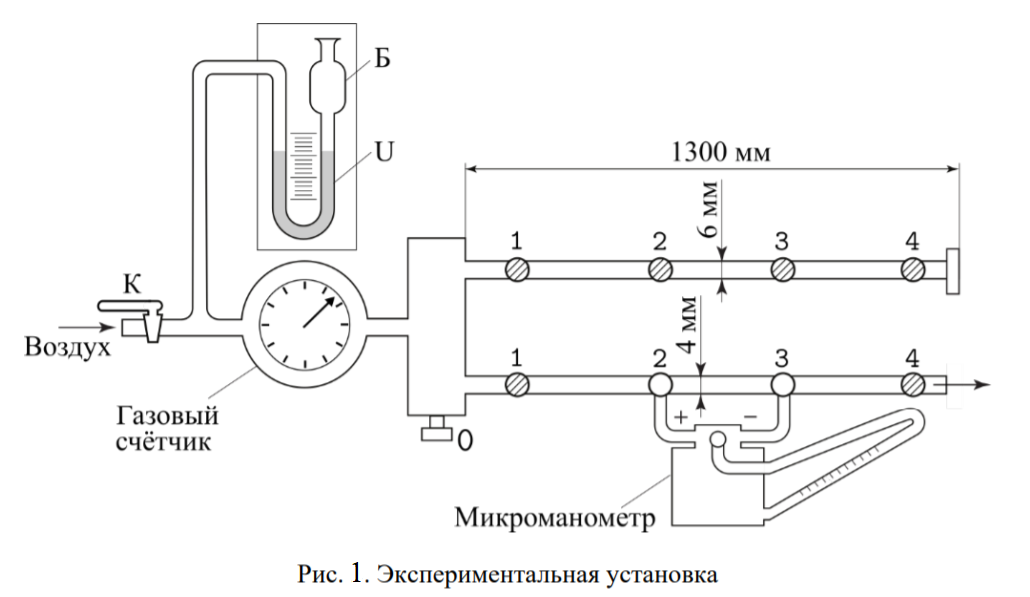
\includegraphics[width = \textwidth]{Рисунок 1.png}
    \end{center}
    
    \subsection{Общая информация}
    Схема экспериментальной установки приведена на рисунке 1. Поток воздуха под давлением, немного превышающем атмосферное, поступает через газовый счётчик в тонкие металлические трубки. Воздух нагнетается компрессором, интенсивность подачи регулируется краном К. Трубки снабжены съёмными заглушками на концах и рядом отверстий, к которым можно подключить микроманометр.
    
    Перед входом в газовый счётчик установлен водяной U-образный манометр. Он предназначен для измерения давления газа на входе, а также предохраняет счётчик от выхода из строя. При превышении максимального избыточного давления на входе счётчика ($\sim$ 30 см вод. ст.) вода выплёскивается из трубки в защитный баллон Б, создавая шум и привлекая к себе внимание экспериментатора.
    
    \subsection{Газовый счётчик}
    \begin{wrapfigure}{r}{0.35\textwidth}
        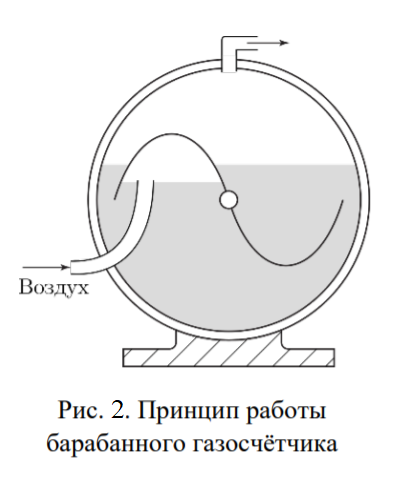
\includegraphics[width = 0.35\textwidth]{Рисунок 2.png}
    \end{wrapfigure}
    В работе используется газовый счётчик барабанного типа. Он позволяет измерять объём газа, прошедшего через систему за некоторое время. Работа счётчика основана на принципе вытеснения: на цилиндрической ёмкости жёстко укреплены лёгкие чаши, в которые поочередно поступает воздух из входной трубки расходомера. Когда чаша наполняется, она всплывает и её место занимает следующая и т.д. Вращение оси предаётся на счётно-суммирующее устройство.
    
    \subsection{Микроманометр}
    В работе используется жидкостный манометр с наклонной трубкой. Разность давлений на входах манометра измеряется по высоте подъёма рабочей жидкости (в данной работе: этилового спирта). Регулировка наклона позволяет измерять давление в различных диапазонах. На крышке прибора установлен трехходовой кран, имеющий два рабочих положения — (0) и (+). В положении (0) производится установка мениска жидкости на ноль. В положении (+) производятся измерения.
    
\section{Методика измерений}	

    Для проведения основных измерений необходимы также подготовительные. Необходимо рассчитать расход воздуха, соответствующий критическому значению числа Рейнольдса, используя табличное значение вязкости ($\eta \sim 2\cdot 10^{-5}\text{ Па}$). Затем, используя формулу Пуазёйля \eqref{puaz}, необходимо получить соответствующий перепад давлений и выразить результат в единицах шкалы микроманометра. Также следует оценить длину $l_{\text{уст}}$ по формуле \eqref{length}.
    
    Основываясь на полученных значениях, в ходе измерений нужно выбирать участки трубы длина которых превышает $l_{\text{уст}}$. Перепад давлений для измерений в условиях ламинарного течения не должен превышать $\Delta P_{\text{кр}}$.
    
\section{Приборы и инструментальные погрешности}

    Давление из единиц микроманометра в паскали переводилось согласно формуле:
    \[\Delta P = 0,2\cdot9,81\cdot\frac{0,8031}{0,8095}\cdot h,\]
    где $h$ - показания микроманометра в миллиметрах, $\Delta P$ - перепад давления в паскалях. За погрешность $h$ принималась половина цены деления, то есть $0,5\text{ мм}$.
    
    Время измерялось с помощью секундомера, установленного на смартфон. Его погрешность пренебрежимо мала, но в качестве погрешности измерения времени возьмём $0,5\text{ с}$, как характерное время реакции человека.
    
    Поскольку класс точности газового счётчика равен 1, а максимально значение на шкале - $5\text{ л}$, то его абсолютная погрешность равна $0,05\text{ л}$. 

\section{Обработка полученных результатов}

    \subsection{Получение коэффициента вязкости}
    Была проведена серия из 7 измерений зависимости $Q(\Delta P)$ для ламинарного течения и 6 - для турбулентного. Измерения проходили на участке трубы длиной 50 см; сама труба имеет диаметр $d = 3,95 \pm 0,05\text{ мм}$. Результаты измерений представлены в таблице 1. По этим данным построены графики: график 1, содержащий точки, соответствующие ламинарному течению, и график 2, содержащий точки, соответствующие обоим видам течения.
    
    Из части таблицы, соответствующей ламинарному течению, с помощью метода наименьших квадратов получаем коэффициент пропорциональности между $Q$ и $\Delta P$.
    \[k\equiv \frac{\pi R^4}{8\eta l} = (640\pm 1)\cdot10^{-9}\frac{\text{м}^3}{\text{с}}\]
    Откуда получаем:
    \[\eta = \frac{\pi R^4}{8k l} = \frac{\pi d^4}{128kl} = 1,87\cdot10^{-5}\text{ Па}\cdot\text{с}\]
    Погрешность вязкости найдём по формуле:
    \[\sigma_{\eta} = \eta\sqrt{\left(\frac{4\sigma_d}{d}\right)^2 + \left(\frac{\sigma_k}{k}\right)^2} = 9\cdot10^{-7}\text{ Па}\cdot\text{с}\]
    Таким образом, окончательно получаем:
    \[\eta = (1,87 \pm 0,09)\cdot10^{-5}\text{ Па}\cdot\text{с}\]
    
    Определим также критическое значение числа Рейнольдса, соответствующее условиям данного опыта. В качестве характерной скорости возьмём среднюю по потоку.
    \[\overline{u} = \frac{Q}{\pi R^2} = \frac{4Q}{\pi d^2}\]
    Поскольку из наблюдений за колебаниями столбика манометра известно, при каком потоке течение перешло в турбулентный режим, в качестве $Q$ возьмём $91,7\ \frac{\text{мл}}{\text{с}}$. Отсюда находим:
    \[\overline{u} = (7,5 \pm 0,1)\ \frac{\text{м}}{\text{с}}\]
    За характерный размер примем радиус трубы, на котором проводились измерения, то есть $r = \frac{1}{2}\cdot 3,95\text{мм}$. Плотность воздуха найдём из законов идеального газа ($T = 25,5 \degree C$, $P = 99490\text{ Па}$; их погрешности неизвестны):
    \[\rho = \frac{\mu P}{RT} = 1,16\ \frac{\text{кг}}{\text{м}^3}\] 
    Окончательно имеем:
    \[Re_{\text{кр}} = 920 \pm 50\]
    
    \subsection{Исследование распределения давления газа вдоль трубки}
    Были проведены измерения давления на 5 участках разной длины двух трубок диаметром $3,95\text{ мм}$ (3 наибольших значения по обеим осям) и $3\text{ мм}$. Результаты измерений приведены в таблице 2. Также по этим данным построен график 3. Сделать вывод о длине участка, на котором устанавливается поток не представляется возможным, так как недостаточно экспериментальных точек между значениями длины 40 и 90 см.
    
    \subsection{Измерение расхода от диаметра трубы при фиксированном градиенте давления}
    Во время выполнения работы удалось провести 3 измерения, относящихся к этому пункту. Их результаты приведены в таблице 3.
    Коэффициент наклона аппроксимирующей прямой: $k = 3.9 \pm 0.2$. Это значение и является той степенью, в которой входит радиус в формулу Пуазёйля.
    
\section{Вывод}
    
    Коэффициент вязкости воздуха с учётом оценённой погрешности соответствует табличных данным. Также с теоретическим расчётом совпадает степень, в которой входи радиус трубы в формулу для объёмного расхода жидкости при ламинарном течении. Однако определить зависимость объёмного расхода от длины трубы не получилось в связи с малым количеством измерений и банальных ошибок экспериментатора (измерения проводились на двух трубах различного радиуса вместо одной).

\newpage
\section{Приложения}

    \subsection{Таблица 1. Измерения зависимости расхода газа от перепада давления}
    \begin{tabular}{|c|c|c|c|c|c|}
        \hline
        h, мм & $\Delta P$, Па & $\sigma_{\Delta P}$, Па & t, с & Q, мл/с & $\sigma_{Q}$, мл/с \\ \hline
        \multicolumn{6}{|c|}{Ламинарное течение}    \\ \hline
        40 & 78  & 1 & 200 & 50,0 & 0,3             \\ \hline
        45 & 88  & 1 & 179 & 55,9 & 0,3             \\ \hline
        50 & 97  & 1 & 160 & 62,5 & 0,4             \\ \hline
        55 & 107 & 1 & 145 & 69,0 & 0,4             \\ \hline
        60 & 117 & 1 & 134 & 74,6 & 0,5             \\ \hline
        65 & 127 & 1 & 123 & 81,3 & 0,5             \\ \hline
        70 & 136 & 1 & 115 & 87,0 & 0,6             \\ \hline
        \multicolumn{6}{|c|}{Турбулентное течение}  \\ \hline
        75  & 146 & 1 & 109 & 91,7  & 0,6           \\ \hline
        105 & 204 & 1 & 98  & 102,0 & 0,7           \\ \hline
        130 & 253 & 1 & 90  & 111,1 & 0,8           \\ \hline
        145 & 282 & 1 & 86  & 116,3 & 0,9           \\ \hline
        200 & 389 & 1 & 74  & 135,1 & 1,1           \\ \hline
        230 & 448 & 1 & 69  & 144,9 & 1,3           \\ \hline
    \end{tabular}
    
    \subsection{Таблица 2. Измерения распределения давления по трубке}
    \begin{tabular}{|c|c|c|c|}
        \hline
        h, мм & $\Delta P$, Па & $\sigma_{\Delta P}$, Па & x, см \\ \hline
        65 & 127 & 1 & 90   \\ \hline
        34 & 66  & 1 & 40   \\ \hline   
        21 & 41  & 1 & 30   \\ \hline
        12 & 23  & 1 & 26,5 \\ \hline
        10 & 19  & 1 & 20   \\ \hline
    \end{tabular}
    
    \subsection{Таблица 3. Измерения зависимости расхода газа от радиуса трубы}
    \begin{tabular}{|c|c|c|c|c|c|}
        \hline
        h, мм & $\Delta P$, Па & $\sigma_{\Delta P}$, Па & t, с & Q, мл/с & $\sigma_{Q}$, мл/с \\ \hline
        50 & 97 & 1 & 274 &  36,5 & 0,2       \\ \hline
        50 & 97 & 1 & 101 &  99,0 & 0,7       \\ \hline
        50 & 97 & 1 &  90 & 111,1 & 0,8       \\ \hline
    \end{tabular}

    \newpage
    \subsection{График 1. Ламинарное течение}
    \begin{center}
        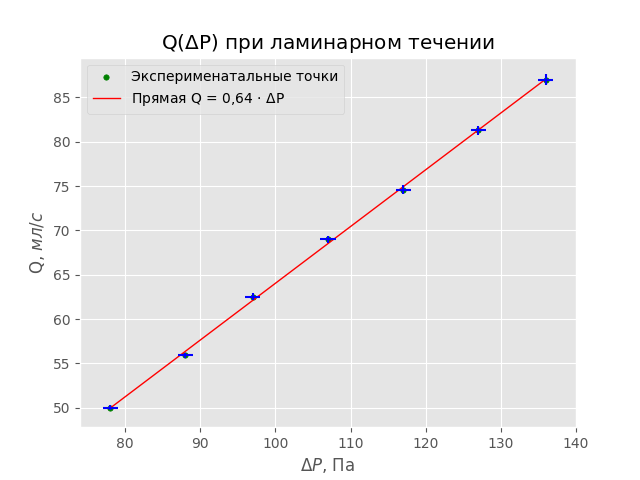
\includegraphics[width = 0.75\textwidth]{График 1.png}
    \end{center}
    
    \subsection{График 2. Ламинарное и турбулентное течения}
    \begin{center}
        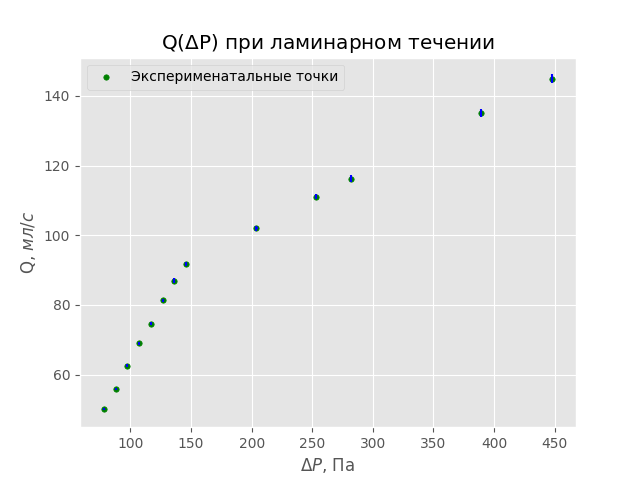
\includegraphics[width = 0.75\textwidth]{График 2.png}
    \end{center}
    
    \subsection{График 3. Распределение давления по трубе}
    \begin{center}
        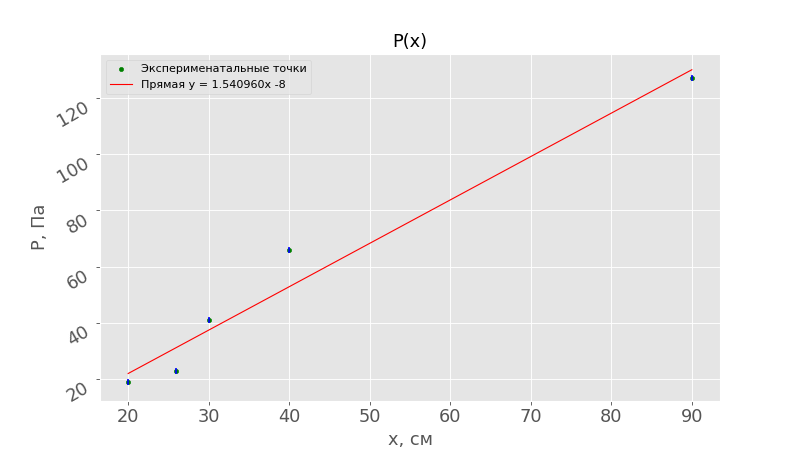
\includegraphics[width = 0.75\textwidth]{График 3.png}
    \end{center}
    
    \subsection{График 4. Зависимость расхода от радиуса трубы}
    \begin{center}
        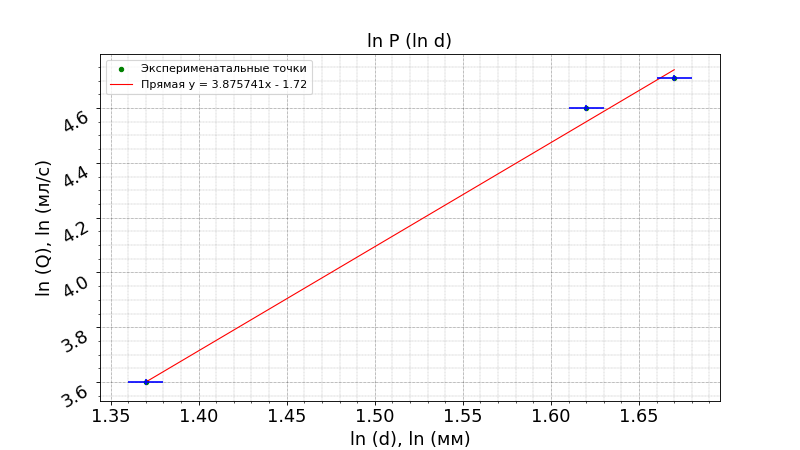
\includegraphics[width = 0.75\textwidth]{График 4.png}
    \end{center}

\end{document}